\documentclass[]{article}
\usepackage{etex}
\usepackage[margin = 1.5in]{geometry}
\setlength{\parindent}{0in}
\usepackage{amsmath}
\usepackage{amsfonts}
\usepackage{amssymb}
\usepackage{amsthm}
\usepackage{listings}
\usepackage{color}
\usepackage{mathtools}
\usepackage{multicol}
\usepackage[lined]{algorithm2e}
\usepackage{float}
\usepackage[T1]{fontenc}
\usepackage{ae,aecompl}
\usepackage[pdftex,
pdfauthor={Michael Noukhovitch},
pdftitle={},
pdfsubject={Lecture notes from },
pdfproducer={LaTeX},
pdfcreator={pdflatex}]{hyperref}

\usepackage{cleveref}
\usepackage{enumitem}

\definecolor{dkgreen}{rgb}{0,0.6,0}
\definecolor{gray}{rgb}{0.5,0.5,0.5}
\definecolor{mauve}{rgb}{0.58,0,0.82}
\DeclareMathOperator*{\argmax}{arg\,max}
\DeclareMathOperator*{\argmin}{arg\,min}

\lstset{
    language=C,
    aboveskip=3mm,
    belowskip=3mm,
    showstringspaces=false,
    columns=flexible,
    basicstyle={\small\ttfamily},
    numbers=none,
    numberstyle=\tiny\color{gray},
    keywordstyle=\color{blue},
    commentstyle=\color{dkgreen},
    stringstyle=\color{mauve},
    breaklines=true,
    breakatwhitespace=true,
    tabsize=4
}

\theoremstyle{definition}
\newtheorem*{defn}{Definition}
\newtheorem{ex}{Example}[section]
\newtheorem*{theorem}{Theorem}

\setlength{\marginparwidth}{1.5in}
\setlength{\algomargin}{0.75em}

\DeclarePairedDelimiter{\set}{\lbrace}{\rbrace}

\definecolor{darkish-blue}{RGB}{25,103,185}

\usepackage{hyperref}
\hypersetup{
    colorlinks,
    citecolor=darkish-blue,
    filecolor=darkish-blue,
    linkcolor=darkish-blue,
    urlcolor=darkish-blue
}
\newcommand{\lecture}[1]{\marginpar{{\footnotesize $\leftarrow$ \underline{#1}}}}

\makeatletter
\def\blfootnote{\gdef\@thefnmark{}\@footnotetext}
\makeatother

\begin{document}
\let\ref\Cref

\title{\bf{Natural Language Processing}}
\date{Fall 2020, McGill\\ \center Notes written from Jackie Cheung's lectures}
\author{Michael Noukhovitch}

\maketitle
\newpage

\tableofcontents

\newpage

\section{Introduction}%
\label{sec:introduction}

\subsection{Overview}%
\label{sub:overview}

\textbf{language} is a form of communication
\begin{itemize}
    \item \textit{arbitrary} pairing between form and meaning
    \item very expressive and productive
    \item nearly universal
    \item uniquely human*
\end{itemize}

\textbf{computational linguistics} modelling natural language with computational models
\begin{itemize}
    \item acoustic signals
    \item NL understanding (comprehension)
    \item NL generation (production)
\end{itemize}

goals of the field
\begin{itemize}
    \item practical technologies (NLP)
    \item understanding how language works (CL)
\end{itemize}

models and techniques
\begin{itemize}
    \item gathering data
    \item evaluation
    \item statistical methods (ML)
    \item rule-based systems
\end{itemize}

some example problems
\begin{itemize}
    \item is language an instinct? (Chomsky)
    \item language processing to understand meaning of sentence
    \item can we learn mathematical properties of language
\end{itemize}

types of language
\begin{itemize}
    \item \textbf{text} an idealization of spoken language
        \begin{itemize}
            \item luckily English is similar between writing and speaking, and there is lots of data on it
            \item older work used ``clean'' language but recent work ventures into messy data (e.g. Twitter)
        \end{itemize}
    \item \textbf{speech} is much messier
        \begin{itemize}
            \item automatic speech recognition (ASR)
            \item text-to-speech generation (TTS)
        \end{itemize}
\end{itemize}

\subsection{Domains of Language}%
\label{sub:domains_of_language}

\textbf{phonetics} study of speech sounds
\begin{itemize}
    \item articulation, transmission
    \item how each sound is made in the mouth
\end{itemize}
\textbf{phonology} rules that govern sound patterns
\begin{itemize}
    \item how the sounds are organized
    \item ``p'' in peach and speach are the same phoneme but phonetically distinct (aspiration)
\end{itemize}
\textbf{morphology} word formation and meaning
\begin{itemize}
    \item anti-dis-establish-ment-arian-ism
\end{itemize}
\textbf{syntax} structure of language
\begin{itemize}
    \item ``I a woman saw park in the'' is \textbf{ungrammatical}
    \item \textbf{ambiguity} different possible meaning for the same phrase
\end{itemize}
\textbf{semantics} meaning of language
\begin{itemize}
    \item ``Ross wants to marry \textbf{a} Swedish woman''
\end{itemize}
\textbf{pragmatics} meaning of language in context
\begin{itemize}
    \item different from literal meaning
    \item \textbf{deixis} interpretation that relies on extra-linguistic context
    \item ``dessert would be delicious''
\end{itemize}
\textbf{discourse} structure of larger spans of language
\begin{itemize}
    \item do large spans of text form a coherent story
\end{itemize}

\subsection{Technology}%
\label{sub:technology}

combination of hand-crafted knowledge and ML on data
\begin{itemize}
    \item rule-based systems
    \item machine learning
    \item knowledge representation
\end{itemize}

\section{Text Classification}%
\label{sec:text_classification}

\subsection{Basics}%
\label{sub:basics}

\textbf{text classification} assign a label or category to a piece of text
\begin{itemize}
    \item sentiment analysis
    \item spam detection
    \item language identification
    \item authorship attribution
\end{itemize}

\textbf{supervised} output data is labelled
\begin{itemize}
    \item learn a function, minimize $\theta$ with loss on data
    \item e.g. spam classificaiton, predict POS
    \item \textbf{regression} $y$ is continuous
    \item \textbf{classification} $y$ is discrete
\end{itemize}
\textbf{unsupervised} output data is unlabelled
\begin{itemize}
    \item learn a density
    \item e.g. grammar induction, word-relatedness (word2vec)
\end{itemize}

\subsection{Building a text classifier}%
\label{ssub:building_a_text_classifier}

\begin{itemize}
    \item define problem, collect data
    \item extract feats
    \item train a classifier on train data
    \item apply classifier to test data
\end{itemize}

problem definition
\begin{itemize}
    \item problem
    \item input
    \item output categories
    \item how to annotate
\end{itemize}

\subsection{Feature Extraction}%
\label{ssub:feature_extraction}


\textbf{feature extraction} get ``important'' properties of documents
\begin{itemize}
    \item convert text into numerical format
    \item e.g. word counts as features \textit{unigram counts}
\end{itemize}

\textbf{lemma} remove affixes get dictionary word ``flies $\to$ fly''
\textbf{stemming} remove affix get stem ``airliner $\to$ airlin''
\begin{itemize}
    \item rule-based e.g. (Porter, 1980) ``ies $\to$ i''
\end{itemize}
\textbf{n-grams} sequences of adjacent words
\begin{itemize}
    \item presence or absence
    \item counts
    \item proportion of total document
    \item scaled version (tf-idf)
\end{itemize}
\textbf{POS tags} crudely capture syntactic pattern (PTB dataset)
\textbf{stop-word removal} remove common uninformative words

sentence representation
\begin{itemize}
    \item vector addition $v_{hello} + v_{world}$
    \item vector multiplication $v_{hello} \cdot v_{world}$
    \item \textbf{max pooling} choose the max of vectors
\end{itemize}


\subsection{Models}%
\label{sub:models}

\textbf{training} select parameters $\theta^*$ according to some objective

types of models
\begin{itemize}
    \item \textbf{generative} models joint distribution $P(x, y)$
        \begin{itemize}
            \item less flexible features as they need to be consistent with each other
        \end{itemize}
    \item \textbf{discriminative} models conditional $P(y|x)$
        \begin{itemize}
            \item can be more flexible in terms of features
        \end{itemize}
\end{itemize}

\subsubsection{Naive Bayes}%
\label{ssub:naive_bayes}

\textbf{Naive Bayes} probabilistic classifier that uses Bayes' Rule $P(y|x) = \frac{P(y)P(x|y)}{P(x)}$
\begin{itemize}
    \item generative
    \item assumes data $x$ is generated independently conditioned on class $P(x_i | y)$
    \item graphical assumption $P(x,y) = P(y) \prod_i P(x_i|y)$
\end{itemize}

In NLP, we can assume NB over a \textit{categorical} distribution and train
\begin{itemize}
    \item loss $L = \prod_{(x,y) \in D} P(y) \prod_i P(x_i|y)$
    \item learn $P(Y=y)$ proportion of samples with class $y$
    \item learn $P(X_i = x| Y= y)$ proportion of samples with feature $x$ given class $y$
\end{itemize}

Inference time we want $P(y|x)$
\begin{align}
    P(y|x) &= P(x,y) | P(x) \\
           &= P(y) \prod_i P(x_i|y) / P(x)
\end{align}
where $P(x)$ is the marginalized over all classes

\subsubsection{Logistic Regression}%
\label{ssub:logistic_regression}

\textbf{logistic regression} linear regression with a logit activation
\begin{itemize}
    \item $P(y|x) = \frac{1}{Z} \exp (\sum_i a_i x_i)$
    \item squash output between $(0,1)$
\end{itemize}

train log-likelihood with \textit{gradient descent}

\begin{align}
    \log L(\theta) &= \prod_{(x,y) \in D} \log P(y|x;\theta) \\
                   &=  \prod_{(x,y) \in D} (\sum_i a_i x_i - \log Z)
\end{align}

\subsubsection{Support Vector Machines}%
\label{ssub:support_vector_machines}

SVM learns linear decision to maximize margin to nearest sample in each of two classes
\begin{itemize}
    \item can be non-linear using \textit{kernels}
\end{itemize}

\subsubsection{Neural Network}%
\label{ssub:neural_network}

\textbf{Perceptron} logistic regression with Perceptron learning rule
$f(x) = \begin{cases} 1 & \text{if } wx+b > 0 \\ 0 & \text{else} \end{cases}$

\textbf{Stacked Perceptron} stacks perceptron neurons

\textbf{Artificial Neural Network} stacked neurons with non-linear activation functions
\begin{itemize}
    \item can learn complex functions
    \item need lots of data and computational power
    \item given enough neurons can compute any function
    \item highly flexible, generic architecture
    \item \textbf{multi-task learning} train model to solve multiple tasks simultaneously
    \item \textbf{transfer learning} use a network on a task different from its training
\end{itemize}

\textbf{Feed-forward} network
\begin{align}
    h_1 &=  g_1(W_1 x + b_1) \\
    h_2 &=  g_2(W_2 h_1 + b_2) \\
    y &= W_2 h_2
\end{align}

\textbf{Activation function} on the output of a neuron
\begin{itemize}
    \item sigmoid
    \item tanh
    \item ReLU
    \item softmax $\frac{exp(x_i)}{\sum_j \exp(x_j)}$
\end{itemize}

Training neural network done with \textbf{gradient descent} on loss function
\begin{itemize}
    \item \textbf{backpropogation} (Rumelhart et al, 1986) uses chain rule to pass gradient
    \item \textbf{SGD} apply gradient iteratively over mini-batches of data
\end{itemize}


\subsection{Model Selection}%
\label{sub:model_selection}

How to choose preprocessing, model, etc.. evaluate on unseen data!

Data split
\begin{itemize}
    \item \textbf{training} learning the model, 60-90\%
    \item \textbf{dev/validation} evaluating while learning the model
    \item \textbf{testing} evaluate once at the end to see how well you do
\end{itemize}

\textbf{k-fold cross-validation} split training data into $k$ folds, train on $k-1$ fold and test on the last

Evaluation measures
\begin{itemize}
    \item \textbf{accuracy} correct / total samples
    \item \textbf{precision} true positives / all predicted positives
    \item \textbf{recall} true positives / true number of positives
    \item \textbf{F1} $\frac{2 * P * R}{P+R}$, can average with P, R, F1
\end{itemize}

You can average evaluation method across classes
\begin{itemize}
    \item \textbf{macro-average} takes the average after computing P, R, F1 for each class
        \begin{itemize}
            \item $\frac{P_{spam} + P_{not-spam}}{2}$
            \item weighs each \textit{class} equally
        \end{itemize}
    \item \textbf{micro-average} sum of counts first then compute P, R, F
        \begin{itemize}
            \item $P_{micro} = \frac{TP_{spam} + TP_{not-spam}}{AP_{spam} + AP_{not-spam}}$
            \item weighs each \textit{sample} equally
        \end{itemize}
\end{itemize}

key issues
\begin{itemize}
    \item which eval measure to use
    \item stastical significance of test
    \item do these tests matter?
\end{itemize}

\section{Language Modelling}%
\label{sec:language_modelling}

\subsection{Words}%
\label{sub:words}

\textbf{word} smallest unit that can appear in isolation
\begin{itemize}
    \item philosophically not so clear e.g. ``peanut butter'' vs ``football''
    \item practically: \textit{spaces delimit words}
\end{itemize}

word features
\begin{itemize}
    \item \textbf{type} identity of a word (count each word once)
    \item \textbf{token} instance of a word (count number of occurences)
\end{itemize}

counting words
\begin{itemize}
    \item \textbf{term frequency} $TF(w,S) = $number of $w$ in corpus $S$
    \item \textbf{relative frequency} $RF(w,S) = \frac{TF(w,S)}{|S|}$
\end{itemize}

\textbf{corpus} of text to use, e.g.
\begin{itemize}
    \item Brown
    \item British National Corpus
    \item WSJC
\end{itemize}

\textbf{Zipf's law} on the ``long tail'' $f \propto \frac{1}{r}$
\begin{itemize}
    \item frequency of  word is inversely proportional to its rank (by frequency in the corpus)
    \item 100th most common word appears 100x less than most common word
    \item \textbf{Zipf-Mandelbrot} $f = \frac{P}{(r + \rho)^B}$
    \item proportion differs by language
\end{itemize}


\subsection{N-gram Language Models}%
\label{sub:ngram_language_models}

\textbf{language modelling} predicting the next word in a context $P(W = w| C)$
\begin{itemize}
    \item can break down with chain rule $P(w_1,2) = P(w_2|w_1)P(w_1)$
    \item should assign higher probability to grammatical sentence
    \item shouldn't be used to predict grammaticality
    \item captures linguistic knowledge and maybe facts about world
\end{itemize}

\textbf{n-grams} feature using $N-1$ previous words as context using MLE
\begin{itemize}
    \item \textbf{unigram} 1 word, $P(cats) = \frac{\text{count(cats)}}{\text{count(all words}}$
    \item \textbf{bigram} 2 word $P(cats | the) = \frac{\text(counts(the cats)}{\text{count(the)}}$
    \item \textbf{trigram} $N=3$ word context
\end{itemize}

evaluation measure
\begin{itemize}
    \item \textbf{likelihood} of generating the test corpus
    \item \textbf{cross-entropy} $H(p, q) = - \sum_i p_i \log_2 q_i$ with model distribtuion $q$
        \begin{itemize}
            \item information $I(x) = \log_2 \frac{1}{P(x)}$
            \item entropy $H(p) = -\sum_i p_i \log_2 p_i$
            \item approx cross entropy with $H(p,q) = -\frac{1}{N} \log_2 q(w_1,\ldots, w_N)$
        \end{itemize}
    \item \textbf{perplexity} $2^{H(p,q)}$ to make differences larger
\end{itemize}


\subsubsection{Learning}%
\label{ssub:learning}


\textbf{maximum likelihood estimation} choose parameters $\theta$ to maximize likelihood training corpus $X$
\begin{itemize}
    \item i.i.d assumption of words in corpus $P(C;\theta) = \prod_n P(x_n;\theta)$
    \item for a Bernoulli $P(C;\theta) = \theta^{N_1}(1-\theta)^{N_0} \ldots \theta_{MLE} = \frac{N_1}{N_0 + N_1}$
\end{itemize}

two issues with learning
\begin{itemize}
    \item \textbf{overfitting} with high train accuracy, low test data accuracy
    \item \textbf{underfitting} low train accuracy
\end{itemize}

model complexity tradeoff
\begin{itemize}
    \item highly expressive models overfit easier
    \item choose a model class and regularization/smoothing technique
\end{itemize}


\subsubsection{Smoothing}%
\label{ssub:smoothing}

out-of-vocabulary (OOV) at test time is a real problem

simple solution
\begin{itemize}
    \item replace all words less than freq threshold with \texttt{<UNK>}
    \item treat \texttt{<UNK>} as a vocabulary item
\end{itemize}

\textbf{smoothing} probability distribution, move mass to unseen cases
\begin{itemize}
    \item don't trust frequency counts entirely
    \item no longer doing MLE but can use $\theta_{MLE}$ prior
    \item $\theta_{smooth} = \max_\theta P(X;\theta)P(\theta) $
\end{itemize}

\textbf{add-$\delta$ smoothing} add frequency to each word ( \textit{pseudocount}(
\begin{itemize}
    \item for unigram $P(w) = \frac{count(w) + \delta}{N+\delta *|Lexicon|}$
    \item with $\delta=1$ called \textbf{laplace discounting}
\end{itemize}

\textbf{interpolation} lower $N$ in $N$-gram to alleviate data sparsity
\begin{itemize}
    \item combine $\hat P = \lambda_1 P_{unigram}^{MLE} + \lambda_2 P_{bigram}^{MLE} + \lambda_3 P_{trigram}^{MLE}$
\end{itemize}

\textbf{Good-Turing Smoothing} assume probability based on zipf's law, assuming all UNK appear once and readjust others accordingly
\begin{itemize}
    \item build a histogram of event frequency $f_c$ (e.g. 1000 words appear once $f_1 = 1000$, 600 words appear twice $f_2 = 600$)
    \item total number of observed event-tokens $N = \sum_i f_i * i$
    \item $w_c$ is event that occurs $c$ times
    \item choose probability for all unseen $P(UNK) = \frac{f_1}{N}$
    \item readjust other mass $c^* = \frac{(c+1)f_{c+1}}{f_c},P(w_c) = \frac{c^*}{N}$
\end{itemize}

\textbf{GT-refinement} estimate linear regression $f_c^{LR} = a \log c + b$ for higher values of $c$
\begin{itemize}
    \item Good-Turing fails for higher $c$ where $f_{c+1} = 0$
    \item use linear regression estimate for $c >$ threshold
    \item use regular $f_c$ for $c < $ threshold
\end{itemize}

\subsection{Hidden Markov Models}%
\label{ssec:hidden_markov_models}

\subsubsection{POS Tagging}%
\label{ssub:pos_tagging}

\textbf{part of speech} syntactic category that tells you grammatical properties of a word
\begin{itemize}
    \item nouns
    \item verbs
    \item adjectives
    \item prepositions
    \item adverbs
    \item determiners ``the, a, an''
\end{itemize}

other POS
\begin{itemize}
    \item modals and auxiliary verbs ``*did* you see him?''
    \item conjunctions ``and, or, but, yet''
    \item particles ``look *up* and *down*''
\end{itemize}

classes of POS
\begin{itemize}
    \item open class: where new words (\textbf{neologism}) can be added to the language
        \begin{itemize}
            \item e.g. nouns like "Kleenex", adjectives like "sick"
            \item tend to be content words
        \end{itemize}
    \item closed class: new words \textit{tend} not to be added
        \begin{itemize}
            \item function words that convey grammatical info
        \end{itemize}
\end{itemize}

corpora
\begin{itemize}
    \item Penn Treebank (45 tags)
    \item Brown corpus (87 tags)
\end{itemize}

language differences
- japanese doesn't differ between nouns and pronouns but verbs are closed class
- wolof doesn't conjugate verbs for person and tense but pronouns are
- Salishan languages may not distinguish between nouns and verbs

POS tagging is a \textbf{sequence labelling} problem since it uses context

\subsubsection{Markov Chains}%
\label{ssub:markov_chains}

We assume a \textbf{markov process}
\begin{itemize}
    \item $N$ states
    \item weighted transitions between states
    \item transition only dependent on current state
\end{itemize}

Model POS as \textbf{hidden variable} aka state, words are visible \textbf{emissions}
\begin{itemize}
    \item independence assumption allows you to factorize
    \item $P(O,Q) = P(Q_1) \prod_t P(Q_{t+1}|Q_t) \prod_t P(O_t | Q_t)$
    \item $P(the text) = P(DT) P(the | DT) P(NN | DT) P (text | NN)$
\end{itemize}

HMM for $N$ tags, $W$ words, parameters $\theta$
\begin{itemize}
    \item initial prob $Q_1$
    \item transition probs $a_{t,t+1}: Q_t \to Q_{t+1}$
    \item emission probs $b_t(O_t): Q_t \to O_t$
\end{itemize}


Choosing the most likely POS tag for each output is naive!
\begin{itemize}
    \item $P(O|\theta)$ computing likelihood of a sequence (forward/backward algorithm)
    \item $\argmax_Q P(Q, O|\theta)$ what state sequence best explains observations (Viterbi)
    \item Given an observation sequence, what is the best model? (Forward-Backward, Baum-Welch, EM)
\end{itemize}

\subsubsection{Forward Algorithm}%
\label{ssub:forward_algorithm}

$P(O|\theta) = \sum_Q P(O,Q|\theta)$

since there are $N^T$ possible paths so use DP to avoid recalculations (see Trellis in \ref{fig:forward-trellis})

\begin{figure}[h]
    \centering
    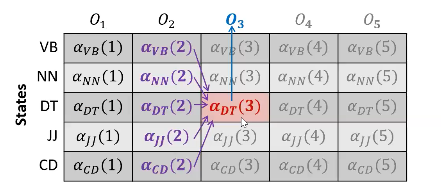
\includegraphics[width=0.8\linewidth]{comp550/forward.png}
    \caption{Trellis for Forward Algorithm}%
    \label{fig:forward-trellis}
\end{figure}

Current tag,previous words given previous tags $\alpha_i(t) = P(O_{1:t},Q_t = i | \theta)$
\begin{itemize}
    \item initial prob $\alpha_j(1) = \pi_j b_j(O_1)$
    \item recurrent sum over prev $\alpha_j(t) = \sum_i \alpha_i(t-1) a_{ij} b_j(O_t)$
    \item final $P(O|\theta) = \sum_j \alpha_j(T)$
    \item runtime $O(N^2T)$
\end{itemize}

\subsubsection{Backward Algorithm}%
\label{ssub:backward_algorithm}

Subsequent words given current tag $\beta_(t) = P(O_{t+1:T} | Q_t = i, \theta)$
\begin{itemize}
    \item excludes the current word unlike $\alpha$
    \item initial prob $\beta_j(T) = 1$
    \item recurrent sum over prev $\beta_i(t) = \sum_j a_{ij} b_j(O_{t+1}) \beta_j(t + 1) $
    \item final $P(O|\theta) = \sum_i \pi_i b_i(O_i) \beta_i(1)$
    \item runtime $O(N^2T)$
\end{itemize}

\subsubsection{Forward-Backward}%
\label{ssub:forward_backward}


Double-check forward using backward
\begin{itemize}
    \item $\alpha_i(t) \beta_i(t) = P(O, Q_t = i | \theta)$
    \item therefore $P(O | \theta) = \sum_i \alpha_i (t) \beta_i (t)$ for any $t \in [1\ldots T]$
\end{itemize}

Work in log probs for numerical stability
\begin{itemize}
    \item $\prod p_i \to \sum \log p_i$
    \item $\sum p_i \to \log \sum p_i = b + \log \sum e^{a_i - b}$ where $b = \max \log p_i$
\end{itemize}

\subsubsection{Viterbi}%
\label{ssub:viterbi}

Find most likely state sequence $Q* = \argmax_Q P(Q,O|\theta)$, like forward algorithm, but take the $\max$
\begin{itemize}
    \item initial $\delta_j(1) = \pi_j b_j(O_1) \forall j \in [1,N]$
    \item recurrence $\delta_j(t) = \max_i \delta_i (t-1) a_{ij} b_j(O_t)$
    \item final $\max_i \delta_i(T)$
    \item runtime $O(N^2T)$
\end{itemize}

Recover best $i$ for each $T$ by keeping track of $\argmax_i$ (\ref{fig:viterbi-alg})

\begin{figure}[ht]
    \centering
    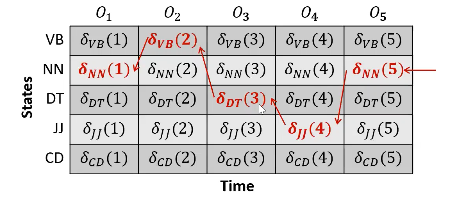
\includegraphics[width=0.8\linewidth]{comp550/viterbi.png}
    \caption{Viterbi backpointers}
    \label{fig:viterbi-alg}
\end{figure}

\subsubsection{Baum-Welch}%
\label{ssub:baum_welch}

How to deal with unsupervised learning? \textbf{Hard EM} or Viterbi EM
\begin{enumerate}
    \item initialize randomly
    \item predict current state sequence using current model
    \item update current parameters based on current predictions
    \item repeat from 2
\end{enumerate}

\textbf{Baum-Welch} or soft EM uses soft predictions
\begin{itemize}
    \item expectation: get expected counts for hidden structures using $\theta_k$
    \item maximization: find $\theta_{k+1}$ to maximize likelihood on expected counts
    \item finds a local optimum in $P(O|\theta)$
\end{itemize}

Expectation of \textbf{responsabilities}: prob distribution over tags
\begin{itemize}
    \item state prob $\gamma_i(t) = P(Q_t = i|O, \theta^k) = \frac{\alpha_i(t)\beta_i(t)}{P(O|\theta^k)} $
    \item transition prob $\xi_{ij}(t) = P(Q_t = i, Q_{t+1} = j| O, \theta^k) = \frac{\alpha_i(t) a_{ij} b_j(O_{t+1})\beta_j(t+1)}{P(O|\theta^k)} $
\end{itemize}

Maximization of Soft MLE update
\begin{itemize}
    \item $\pi_i^{k+1} = \gamma_i(1)$
    \item $a_{ij}^{k+1} = \frac{\sum_t \xi_{ij}(t)}{\sum_t \gamma_i(t)} \approx \frac{count(i,j)}{count(i)} $
    \item $b_i^{k+1}(w_k) = \frac{\sum_t \gamma_{ij}(t)|_{O_t = w_k}}{\sum_t \gamma_i(t)} \approx \frac{count(w_k, i)}{count(i)}$
\end{itemize}

Practical training
\begin{itemize}
    \item stop iteration using performance on held-out set
    \item \textbf{random restarts} train different models from different inits
    \item biased initialization using some external supervised knowledge
    \item \textbf{semi-supervised} with small labelled data and large unlablled
\end{itemize}

\subsubsection{Multiword Tasks}%
\label{ssub:multiword_tasks}

Similar HMM tasks can require multiple words per tag
\begin{itemize}
    \item \textbf{Chunking} find syntactic chunks e.g. \texttt{[The chicken] [crossed] [the road]}
    \item \textbf{Named Entity Recognition} (NER) identify elements corresponding to high-level categories e.g. \texttt{[McGill University] is located in [Montreal, Canada]}
\end{itemize}

\textbf{IOB tagging} label whether word is at beginning, inside, or outside a span of tags e.g. McGill\texttt{[B-ORG]} University\texttt{[I-ORG]} is located in Montreal\texttt{[B-LOC]} Canada\texttt{[I-LOC]}

\subsection{Linear-chain CRF}%
\label{ssub:linear_chain_crf}

\subsubsection{Discriminative}%
\label{ssub:discriminative}


Shortcoming of HMMs
\begin{itemize}
    \item adding a feature requires adding an emission e.g. word position, capitalization...
\end{itemize}

\textbf{LC-CRF} linear chain conditional random field
\begin{itemize}
    \item HMM-like task-specific discriminative model $P(Y|X;\theta)$ using features, not probs
    \item $P(Y|X) = \frac{1}{Z(X)} \exp \sum_t \sum_k \theta_k f_k(y_t, y_{t-1}, x_t)$
    \item $Z(X) = \sum_y P(Y|X)$ is a normalization constant
    \item sum over all timesteps $t$, features $k$
\end{itemize}

Examples of features
\begin{itemize}
    \item HMM probs e.g. emit "the" from DT $1(y_t = DT) 1(x_t = "the")$
    \item capitalization $1(y_t = ?) 1(x_t \text{is capitalized})$
\end{itemize}


\subsubsection{Inference}%
\label{ssub:inference}

Forward algorithm computes $Z(X)$
\begin{itemize}
    \item initial prob $\alpha_j(1) = \exp \sum_k \theta_k^{init} f_k^{init}(y_1 = j, x_1)$
    \item recurrent sum over prev $\alpha_j(t) = \sum_i \alpha_i(t-1)\exp \sum_k \theta_k f_k(y_t = j, y_{t-1}, x_1) $
    \item final $Z(X) = \sum_j \alpha_j(T)$
\end{itemize}

Viterbi algorithm computes $\argmax_Y P(Y|X,\theta)$


\subsubsection{Training}%
\label{ssub:training}

Use gradient descent $\theta_{t+1} \gets \theta_t + \alpha \nabla l(\theta)$
\begin{itemize}
    \item no analytic solution
    \item $l(\theta)$ is concave
    \item can use conjugate gradient and L-BFGS
\end{itemize}

Gradient $\nabla l(\theta)$ = empirical count of features - expected feature count using current model
\begin{itemize}
    \item minimized when model matches empirical distribution
    \item regularization $\sum_k \frac{\theta_k^2}{2\sigma^2}$
    \item SGD used in practice
\end{itemize}

\subsection{Recurrent Neural Networks}%
\label{sub:recurrent_neural_networks}

\subsubsection{Neural Networks}%
\label{ssub:neural_networks}

Feed-forward NN
\begin{itemize}
    \item all computations flow forward
\end{itemize}

Time-delay NN
\begin{itemize}
    \item feed context window around word into FF
    \item requires fixed horizon
    \item sequence interaction learned indirectly, not sequence model!
\end{itemize}

\subsubsection{RNN}%
\label{ssub:rnn}

RNN: NN sequence model
\begin{itemize}
    \item modelling long-range dependencies
    \item $RNN(s_0, x_{1:n}) = s_{1:n}, y_{1:n}$
    \item $s_i = R(s_{i-1}, x_i)$
    \item $y_i = O(s_i)$
\end{itemize}

comparison to LC-CRF
\begin{itemize}
    \item LCCRF is linear, RNN is more expressive
    \item LCCRF uses feature engineering, RNN discovers features
    \item LCCRF assumes local independence, fast inference, RNN need approx (e.g. beam-search)
\end{itemize}


\subsubsection{LSTM}%
\label{ssub:lstm}

vanishing and exploding gradient
\begin{itemize}
    \item gradients wrt time 1 $ \frac{\partial L}{\partial W^1} =
        \frac{\partial L}{\partial f^N}
        \frac{\partial f^{N-1}}{\partial f^{N-2}} \ldots
        \frac{\partial f^1}{\partial W^1} $
    \item if gradient norm $<1$, it will vanish
    \item if gradient norm $>1$, it will explode to infinity
\end{itemize}

Long Short-Term Memory (Hochreiter and Schmidhuber, 1997)
\begin{itemize}
    \item explicitly model memory $C_t = f_t * C_{t-1} + i_t * \tilde C_t$
    \item forget $f_t = \sigma(W_f \cdot [h_{t-1},x_t]) $
    \item input $i_t = \sigma(W_i \cdot [h_{t-1},x_t]), \tilde C = \tanh (W_C \cdot [h_{t-1}, x_t])  $
    \item output $o_t = \sigma(W_o \cdot [h_{t-1},x_t])$
        $h_t = o_t * \tanh(C_t)$
\end{itemize}

BiLSTM, a layer for forward and backward
\begin{itemize}
    \item concatenate $h_{forward},h_{backward}$ to get output
\end{itemize}

LSTM-CRF, LCCRF layer on top of a BiLSTM
\begin{itemize}
    \item using features: output scores of LSTM $P$, transition probabilities b/w tags (learned) $A$
    \item total score $s(X,y) = \sum_i A_{y_i,y_{i+1}} + \sum_i P_{i,y_i}$
\end{itemize}

training
\begin{enumerate}
    \item forward pass for BiLSTM
    \item forward CRF to get predictions
    \item backward pass CRF to get loss
    \item backprop loss through BiLSTM
\end{enumerate}

\subsection{Pretrained LMs}%
\label{sub:pretrained_lms}

\subsubsection{Transfer Learning}%
\label{ssub:transfer_learning}

\textbf{transfer learning} using knowledge from one task to improve performance on another
\begin{itemize}
    \item don't start task from scratch, transfer knowledge of words, syntax,...
    \item use language modelling as a source task
\end{itemize}

ELMo (Peters et al, 2018) large-scale LM pretrained BiLSTM
\begin{itemize}
    \item generate contextual word embeddings
    \item $ELMo(w_k)$ = weighted sum of BiLSTM layers
\end{itemize}

\subsubsection{Transformer}%
\label{ssub:transformer}

Attention is all you need (Vaswani et al, 2017)
\begin{itemize}
    \item allow information flow between any pair of words
    \item Transformer architecture uses only attention, no recurrence
    \item $O(N^2)$ connections but better parallelism
\end{itemize}

attention, three views of a word
\begin{itemize}
    \item query: word we want to compute in the next layer
    \item key: how important the word is to another word
    \item value: value associated with the key once attention is computed
\end{itemize}


\subsubsection{Large Scale Pretrained Models}%
\label{ssub:large_scale_pretrained_models}


BERT - transformer encoder model
\begin{itemize}
    \item pretraining MLM (masked language modelling) and next sentence prediction
    \item trained on ~3B words
    \item 340M parameters
\end{itemize}

GPT-3 (OpenAI, 2020) - transformer decoder model
\begin{itemize}
    \item pretraining on language modelling
    \item trained on ~500B words
    \item up to 175B model parameters
    \item success in 0-shot and few-shot learning
\end{itemize}

Problems
\begin{itemize}
    \item generated text can be incoherent or repetitive
    \item reasoning about physics + commonsense
    \item arguments about memorization vs understanding
    \item misuse of language models (spam, fake news)
    \item fairness, bias, cost!
\end{itemize}

\section{Syntax}%
\label{sec:syntax}

\subsection{Form of Language}%
\label{sub:form_of_language}


\textbf{syntax} words arranged to form a grammatical sentence
\begin{itemize}
    \item generate all and exactly those sentences which are grammatical ( \textbf{grammaticality} )
    \item \textbf{descriptive} not \textbf{prescriptive}
\end{itemize}

\textbf{contituency} group of words that behave as a unit, e.g for noun phrases
\begin{itemize}
    \item can appear in similar syntactic envs
    \item can be replaced as a unit or rearranged
    \item can be used to answer a question
\end{itemize}
\textbf{grammatical relations} between contituents e.g.
\begin{itemize}
    \item subject
    \item (direct) object e.g. he kicked \textit{the ball}
    \item indirect object e.g. she gave \textit{him} a good beating
\end{itemize}
\textbf{subcategorization} different number and type of args mandatory for a verb or adj
\begin{itemize}
    \item (subj) relax
    \item (subj) steal (obj)
    \item (subj) want (obj / inf clause)
    \item different (from / than / to)
\end{itemize}


\subsection{Formal Grammars}%
\label{sub:format_grammars}

\textbf{formal grammar} rules that generate a set of strings to make up a language

\textbf{finite state automata} generates a regular language
\begin{itemize}
    \item correspond to \textbf{regular grammars}
    \item used for stemming, lemmatization, ...
\end{itemize}

\textbf{context-free grammars} more powerful class of grammars for NL
\begin{itemize}
    \item $N$ set of \textbf{non-terminals}
    \item $\Sigma$ of \textbf{terminals}
    \item $R$ set of rules or productions
    \item $S \in N$ start symbol
\end{itemize}

generation
\begin{itemize}
    \item \textbf{undergeneration} misses valid sentences
    \item \textbf{overgeneration} adds extra invalid sentences
    \item allows recursion
\end{itemize}

\textbf{constituency} grammars combine into bigger and bigger constituents (NP $to$ Det, N)
\begin{itemize}
    \item can be converted into dependency tree if you know the head of constituent
\end{itemize}
\textbf{dependency} grammar represent relations as directed edges
\begin{itemize}
    \item each phrase has a \textbf{head} word e.g. student \textit{studied} for the exam
    \item easier to extract relations
    \item can be converted to contituency trees if \textbf{projective} (dependecy edges don't cross, freer word order langs)
\end{itemize}

\textbf{chomsky hierarchy}
\begin{itemize}
    \item regular
    \item context-free: can describe English/German but not others
    \item context-sensitive: technically Swiss German bc of cross-serial dependencies
    \item recursively enumerable
\end{itemize}

\subsection{CYK Parsing Algorithm}%
\label{sub:cyk_parsing_algorithm}

\subsubsection{CYK Parsing}%
\label{ssub:cyk_parsing}

\textbf{parsing} given input sentence and CFG, recover all possible parse trees
\begin{itemize}
    \item top-down: start at $S$ and expand (e.g. Earley)
    \item bottom-up: start from input words (e.g. CYK, shift-reduce)
\end{itemize}

\textbf{CYK} (Cocke-Younger-Kasami) bottom-up dynamic programming
\begin{itemize}
    \item convert CFG into Chomsky Normal Form
    \item setup table of contituents
    \item fill in table
    \item use table
\end{itemize}

\textbf{Chomsky Normal Form}: $A \to B,C$ non-terminal, $A \to s$ terminal
\begin{itemize}
    \item reduce non-terminals to 2 $A \to B,C,D$ converts $A \to X1,D$ and$X1 \to B,C $
    \item split non-terminal,terminal $A \to s,B$ converts $A \to X2,B$ and $X2 \to s$
    \item remove single non-terminals $A \to B, B \to \ldots$ converts $A \to \ldots$
\end{itemize}

constituent parse table (see \ref{fig:parse-table})
\begin{itemize}
    \item sentence $w[0], w[1] \ldots w[N-1]$
    \item cell $i,j$ corresponds to span $w[i:j+1]$
    \item cell lists non-terminals that can span those words
\end{itemize}

\begin{figure}[ht]
    \centering
    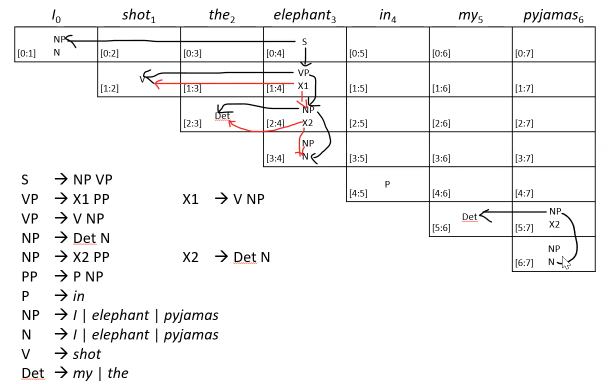
\includegraphics[width=0.7\linewidth]{comp550/parse-table.png}
    \caption{contituent parse table}%
    \label{fig:parse-table}
\end{figure}

build parse table
\begin{itemize}
    \item base: for each word $i$ put in $c[i:i+1]$ non-terminal that generates the word
    \item recursive: check all break points $m \in [i,j]$ and check for rule $A[i,j] \to B[i:m],C[m:j]$
    \item fill in bottom-up, left-to-right
\end{itemize}

use table
\begin{itemize}
    \item use cell $c[0:N]$ and follow back-pointers
\end{itemize}

\subsubsection{Probabilistic CYK Parsing}%
\label{ssub:probabilistic_cyk_parsing}

\textbf{probabilistic CYK} associate each rule with a probability, use product of probabilities for rules
\begin{itemize}
    \item for each non-terminal $A, \sum_B Pr(A \to B) = 1$
    \item combining rules for tree  $t, Pr(t) = \prod_i Pr(A_i \to B_i)$ with rules $A_i \to B_i$
\end{itemize}

\textbf{probabilistic parsing} recovers best parse $\argmax_t Pr(t)$
\begin{itemize}
    \item naive: run CYK and take argmax
    \item idea: keep track of probability in CYK and always choose highest probability parse
\end{itemize}

\textbf{probabilistic CYK} keeps track of probability and only most likely for each tree type
\begin{itemize}
    \item table[2, 4, NP] = 0.215 (table[2,3,Det], table[3,4,N])
    \item table[3, 4, NP] = 0.022
    \item table[3, 4, N] = 0.04
\end{itemize}

\textbf{Vanilla PCFG} learn probabilities using MLE on corpus (e.g. WSJ)
\begin{itemize}
    \item not enough context e.g. "I" "me" are NP but are object or subject
    \item rules are too sparse e.g $VP \to VBD$ and $VP \to VBD,PP$ are separate not factorizable
    \item strong \textit{vertical} assumption, contituent independent of other parts of tree
    \item weak \textit{horization} assumption, tries to model all combinations separately
\end{itemize}

\subsubsection{Markovization}%
\label{ssub:markovization}

Improved PCFG by markovization: better context annotation and factorization
\begin{itemize}
    \item \textbf{vertical} annotate with $n$-th parent $NP^S$ likey subject, $NP^{VP}$ likely object
    \item \textbf{horizontal} factorize large rules like $n$-gram $Pr(VP \to START,AdvP,VBD \ldots) = Pr(VP \to START,AdvP) * Pr(VP \to AdvP,VBD) \ldots$ and learn factors separately
\end{itemize}

WSJ results by Klein and Manning (2003) show large improvement $71.3 \to 79.7$


\section{Semantics}%
\label{sec:semantics}

\subsection{Meaning of Language}%
\label{sub:meaning}

\textbf{semantics} study of meaning in language
\begin{itemize}
    \item \textbf{extensional} picks out word's \textbf{referents} in the real world
    \item \textbf{intensional} defines a word in terms of other words e.g. dictionary
\end{itemize}

Frege (1892) differentiates sense and reference
\begin{itemize}
    \item \textbf{sense} of a term is its meaning, whereas
    \item \textbf{reference} is what it points to in the real world
\end{itemize}

\subsection{Lexical Semantics}%
\label{sub:lexical_semantics}

\textbf{lexical semantics} the meaning of words, with relations
\textbf{hyponym / hypernym} hypo "is a" hyper
\begin{itemize}
    \item class: monkey / mammal
    \item instance: Montreal / city
\end{itemize}
\textbf{synonym} same meaning
\textbf{antonym} opposite meaning
\textbf{homonym} same form, different unrelated meaning
\begin{itemize}
    \item homophone: same sound
    \item homograph: same written form
\end{itemize}
\textbf{polysem} multiple related meanings
\textbf{metonym} substituting one entity for related one (e.g. order a \textit{dish} from the menu)
\begin{itemize}
    \item synecdoche: whole-part relation (e.g. all \textit{hands} on deck)
\end{itemize}
\textbf{meronym / holonym} mero "is part of" holo
\begin{itemize}
    \item groups and members (student / class)
    \item whole and part (wheel / car)
    \item whole and substance (wood / chair)
\end{itemize}


WordNet (Miller et al, 1990) lexical resource organized by \textbf{synsets}
\begin{itemize}
    \item hierarchies based on lexical relations
\end{itemize}

\subsubsection{Word Sense Disambiguation}%
\label{ssub:word_sense_disambiguation}

\textbf{word sense disambiguation} figure out which sense a word is expressing using contextual words

\textbf{Lesk's algorithm} (1986) heuristic approach
\begin{enumerate}
    \item construct $B$ bag-of-words rep for context
    \item calculate $overlap(B, signature(s_i)$ for each candidate sense $s_i$
    \item choose sense with highest overlap
\end{enumerate}

\textbf{Yarowsky's algorithm} (1990) unsupervised (or minimal) based on bootstrapping
\begin{enumerate}
    \item choose word to disambiguate (e.g. plant)
    \item find two senses and label with heuristic (e.g. plant \textit{life} vs \textit{manufacturing}) creating \textit{seed set}
    \item repeat iteration
        \begin{itemize}
            \item learn a supervised model on seed set
            \item predict labels of whole dataset
            \item keep highly confident labels as next seed set
        \end{itemize}
\end{enumerate}

\subsubsection{Hearst Patterns}%
\label{ssub:hearst_patterns}

detect lexical semantic relationships in text since they tend to occur in certain \textbf{lexico-syntactic} patterns

Hearst (1992) patterns for hyper-hypo
\begin{itemize}
    \item NP such as {NP} {and|or} NP
    \item NP {,} including {NP,}
    \item NP {,} especially {NP,}
\end{itemize}

Find new patterns by bootstrapping with known pairs $\to$ patterns $\to$ new pairs

\subsection{Distributional Semantics}%
\label{sub:distributional_semantics}

some semantic rels, e.g. synonyms, do not appear together but rather occur in the same context

``You shall know a word by the company it keeps'' (Firth, 1957)

\subsubsection{Word Vectors}%
\label{ssub:word_vectors}

\textbf{Count-based} word vectors
\begin{itemize}
    \item for some word $i$, keep count of words that appear within a window of $n$ words
    \item generate term-context matrix such as \ref{fig:term-context}
    \item compute cosine sim between word vectors to get similarity
\end{itemize}

\begin{figure}[h]
    \centering
    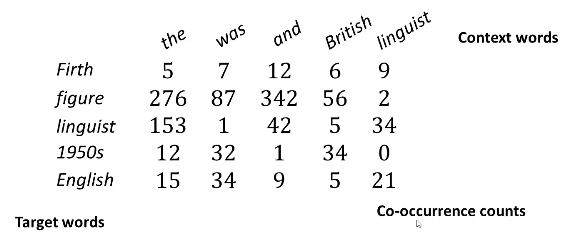
\includegraphics[width=0.6\linewidth]{comp550/term-context.png}
    \caption{term-context matrix}%
    \label{fig:term-context}
\end{figure}

vector similarity measures \textit{relatedness}
\begin{itemize}
    \item synonyms and antonyms are hard to distinguish by context
    \item \textbf{similarity} synonymy, hypernymy, hyponymy
    \item \textbf{relatedness} association, includes antonyms
\end{itemize}

evaluating word vectors is non-trivial
\begin{itemize}
    \item compare to gold standard e.g. WS-353 (Finkelstein et al, 2002)
\end{itemize}

\subsubsection{Better Word Vectors}%
\label{ssub:better_word_vectors}

instead of raw counts use \textbf{Pointwise MI}
\begin{itemize}
    \item $\log \frac{P(w_1,w_2)}{P(w_1)P(w_2)}$
    \item normalizes chance co-occurence
    \item PMI can measure positive correlation $>0$ or negative $<0$
    \item \textbf{Positive PMI} sets $PMI < 0 \to PMI = 0$
\end{itemize}

\subsubsection{Singular Value Decomposition}%
\label{ssub:singular_value_decomposition}

term-context matrices are sparse, compress into smaller dense

\textbf{Singular Value Decomposition} matrix factorization $X = W \times \Sigma \times C^T$
\begin{itemize}
    \item new word vectors $W \in R^{|V| \times m}$
    \item $\Sigma$ has singular values of $X$, arranged highest to lowest
\end{itemize}

\textbf{truncated SVD} take top $k$ values in $\Sigma$
\begin{itemize}
    \item use $W_k \times \Sigma_k$ as word vectors
    \item corresponds to finding smallest reconstruction error
    \item same as PCA, projecting to top $k$ components
\end{itemize}

\subsubsection{Word2Vec}%
\label{ssub:word2vec}

\textbf{word2vec} (Mikolov et al, 2013) trains NNs to predict words in context
\begin{itemize}
    \item vector representations known as \textbf{word embeddings}
    \item CBOW: use context words vec $c_j$ to predict target word vec $v_j$
    \item Skip-gram: use target to predict context $P(w_k | w_j) = \frac{\exp{c_k \cdot v_j}}{\sum_{i \in |V|} \exp{c_i \cdot v_j}}$
    \item \textbf{negative sampling} to approximate denominator, separate true context from fake context
\end{itemize}

hyperparameters are key to performance
- weighting important of context words
- negative sampling $p^{3/4}(w)$ is better than $p(w)$
- similar changes improve other methods like SVD

widely used in NLP
- cheap, easy, large pretrained
- doesn't always work for task-specific

\subsection{Compositional Semantics}%
\label{sub:compositional_semantics}

\subsubsection{Compositionality}%
\label{ssub:compositionality}

\textbf{compositionality} (c) the meaning of a phrase depends on the meaning of its parts
\begin{itemize}
    \item \textbf{non-c} e.g. idioms ``kick the bucket''
    \item \textbf{co-c} meaning depends on composed words e.g. \textit{red} hair vs \textit{red} wine
\end{itemize}

\textbf{c semantics} derivate a good meaning of a representation from its parts
\begin{itemize}
    \item assert a falsifiable proposition
    \item convey information about the world
    \item query about the world
\end{itemize}

\subsubsection{Semantic Inference}%
\label{ssub:semantic_inference}

Montague (1970) used logical formalism to represent meaning

\textbf{semantic inference} make explicit something that is implicit in language (Blackburn and Bos, 2003)

First-order logic
\begin{itemize}
    \item \textbf{domain of discourse} a set of entities
    \item \textbf{variables} potential elements of domain $x$
    \item \textbf{predicates} maps elements to truth value $inCourse(x,y)$
    \item \textbf{functions} maps elements to elements $instructorOf(x) \to y$
    \item \textbf{logical connectives} $\neg, \vee, \wedge, \to \ldots$
    \item \textbf{quantifiers} $\exists, \forall$
\end{itemize}
interpretation or \textbf{model} of a FOL
\begin{itemize}
    \item domain of discourse $D$
    \item mapping of functions to $D$
    \item mapping of predicates to True or False
\end{itemize}

\subsubsection{Lambda Calculus}%
\label{ssub:lambda_calculus}

we need a computation procedure to convert from NL to formal logic

\textbf{lambda calculus}
\begin{itemize}
    \item variable $x$
    \item $\lambda x.t$ where $t$ is a lambda term
    \item $ts$ where both are lambda terms
    \item \textbf{beta reduction} function application of $(\lambda x.t)s$
    \item note that it is \textbf{left associative} $abcd = ((ab)c)d$
\end{itemize}

construct contituents with lambda calculus
\begin{itemize}
    \item ``disdained'' $\lambda x.\lambda y. disdained(y,x)$
    \item ``disdained catnip'' $\lambda y. disdained(y, catnip)$
    \item ``Whiskers disdained catnip'' $(\lambda y. disdained(y, catnip))Whiskers$
\end{itemize}

\textbf{syntax-driven sem composition}: augment CFG with lambda expression
\begin{itemize}
    \item syntax $A \to a_1, \ldots a_n$ semantic attachment $\{f(\alpha_1.sem, \ldots \alpha_n.sem)\}$
    \item common noun $N \to student, \{ \lambda x.Student(x)\}$
    \item proper noun $PN \to COMP550, \{\lambda x.x(COMP550)\}$ \textbf{type-raised} to be same as common
    \item intransitive verb $V \to rules, \{ \lambda x. \exists e Rules(e) \wedge Ruler(e,x) \}$ \\
        \textbf{neo-davidsonian} event semantics $Rules(x)$ uses reified event $e$
    \item composition is function application $S \to NP, VP, \{NP.sem(VP.sem)\} $
\end{itemize}

\subsubsection{Quantification}%
\label{sub:quantification}

quantifiers
\begin{itemize}
    \item universal \textit{all}, $\forall x \ldots \to \ldots$
    \item existential \textit{a}, $\exists x \ldots \wedge \ldots$
    \item definite \textit{the} (Russell, 1905)
        \begin{itemize}
            \item existence $\exists x.Student(x)$
            \item uniqueness (at most one) $\wedge \forall y.Student(y) \to x = y$
            \item predicate $\wedge Smart(x)$
        \end{itemize}
\end{itemize}

more semantic attachments
\begin{itemize}
    \item universal $\lambda P. \lambda Q. \forall x. P(x) \to Q(x)$
    \item existential $\lambda P. \lambda Q. \exists x. P(x) \wedge Q(x)$
    \item adjectives $ \lambda N.\lambda x. Smart(x) \wedge N(x)$
\end{itemize}

\subsubsection{Quantifier Scope Ambiguity}%
\label{ssub:quantifier_scope_ambiguity}

\textbf{scope ambiguity} when multiple quantifier have multiple meanings e.g. ``\textit{Every} student took \textit{a} course''
\begin{itemize}
    \item different course $\forall x.Student(x) \to (\exists y.Course(y) \ldots)$
    \item same course $\exists y.Course(y) \wedge (\forall x.Student(x) \ldots)$
\end{itemize}

\textbf{underspecification} derive representation represents \textit{all possible} meanings

\textbf{Cooper storage} (1988) associates store with each FOL
\begin{align*}
    \exists e.took(e) &\wedge taker(e, \color{red} s_1 \color{black} ) \wedge takee(e,\color{blue}{s_2} \color{black}) \\
                      &(\lambda Q. \forall x.Student(x) \to Q(x), \color{red} 1 \color{black}), \\
                      &(\lambda Q. \exists y.Course(y) \wedge Q(y), \color{blue} 2 \color{black})
\end{align*}

recover reading from cooper storage
\begin{enumerate}
    \item select quantifier order (e.g. $s_1$ first)
    \item do lambda abstraction for each quantifier and apply function (beta-reduce)
\end{enumerate}

\begin{align*}
    \lambda Q. &\forall x.Student(x) \to Q(x) \\
               & \color{red} \lambda s_1 \color{black} \exists e.took(e) \wedge taker(e, \color{red} s_1 \color{black} ) \wedge takee(e,\color{blue}{s_2} \color{black}) \\
                      &(\lambda Q. \exists y.Course(y) \wedge Q(y), \color{blue} 2 \color{black})
\end{align*}


semantic attachment quantifier composition
\begin{itemize}
    \item compose by putting in storage
    \item $NP \to Det, N$ gives $\{ \lambda u.u(\color{red} s_i \color{black}), \text{storage:} (Det.sem(N.sem), \color{red} i \color{black}) \}$
\end{itemize}


\section{Discourse}%
\label{sec:discourse}

\subsection{Language Communication}%
\label{sub:phrases_of_language}

language is a \textit{discourse}
\begin{itemize}
    \item \textbf{monologue} one-directional communication
    \item \textbf{dialogue} multi-participant communication
\end{itemize}

sequential sentences must ``make sense''
\begin{itemize}
    \item \textbf{coherence} is about logical sense
    \item \textbf{cohesion} is about linguistic devices to flow better
        \begin{itemize}
            \item \textbf{lexical chain} of semantically similar words e.g.  The \textit{government} proposes rules. \textit{Citizens} are protesting.
            \item \textbf{anaphoric devices} like \textbf{coreference chains} when one phrase meaning depends on another e.g.  \textit{The rules} are long. \textit{These regulations} \ldots
            \item \textbf{discourse markers} of cue words e.g. The dog is big. Dogs can \textit{also} be small.
        \end{itemize}
\end{itemize}

\subsection{Coreference Resolution}%
\label{sub:coreference_resolution}

\subsubsection{Corefence and Anaphora}%
\label{ssub:corefence_and_anaphora}

\textbf{reference} relating \textit{mentions} to \textit{referents} in the real world
\begin{itemize}
    \item proper names \textit{Montreal}
    \item pronouns \textit{he, she}
    \item noun phrases
        \begin{itemize}
            \item indefinite \textit{a} deer
            \item definite \textit{the} cat
        \end{itemize}
    \item demonstrative: points to something \textit{this} hotdog
\end{itemize}

\textbf{coreference} when two mentions point to the same object
\begin{itemize}
    \item \textbf{anaphor} points to previous Maru is a cat. \textit{He} is grumpy
    \item \textbf{cataphor} points to following When \textit{he} is grumpy, Maru doesn't eat
\end{itemize}

\textbf{zero anaphora} in other \textbf{pro-drop} languages allows omitting pronouns
\begin{itemize}
    \item e.g. Spanish can figure out pronoun using verb \textit{hablo} Español
    \item e.g. Japanese requires context \textit{Ai shi} (love) te ru (prog pres) = I love you
\end{itemize}

noun phrase coreference
\begin{itemize}
    \item \textbf{bridging} infer ref from previous mentions ``I like my office. \textit{The windows} are large''
    \item \textbf{pleonastic} are non-referential pronounce ``\textit{It} is raining''
    \item \textbf{clefting} puts focus on something (sorta referential) ``\textit{It} is my cat that is grumpy''
\end{itemize}

coreference beyond entities and noun phrases
\begin{itemize}
    \item \textbf{event} that corefer or happen in same time / place \\ ``I \textit{bought} my cat. The \textit{adoption} was quick''
    \item \textbf{abstraction} shell noun (this) represents a whole thing  \\ ``Grumpiest cats are the best. \textit{This fact} is true''
    \item \textbf{cross document} alignment of events and entities from multiple sources
\end{itemize}

\subsubsection{Hobbs Algorithm}%
\label{ssub:hobbs_algorithm}

cues for anaphora resolution
\begin{itemize}
    \item number and gender
    \item recency
    \item syntactic info e.g. \textbf{binding theory} (Chomsky, 1981)
        \begin{itemize}
            \item ``the students taught \textit{themselves}''
            \item reflexives are bound by a subject in a certain way
            \item personal pronouns are not
        \end{itemize}
\end{itemize}

Hobbs (1978) traversal algorithm using constituent parse tree and morph analysis of number and gender
\begin{enumerate}
    \item search the sentence right-to-left
    \item use heuristics and check if NP found match in number and gender
    \item if no antecedent found, search previous sentences left-to-right
\end{enumerate}


\subsubsection{Coreference ML}%
\label{ssub:coreference_ml}

coreference subtasks
\begin{itemize}
    \item \textbf{mention detection} decide which text are mentions and anaphoric
    \item \textbf{coreference resolution} determine coref links in passage
\end{itemize}

Soon et al (2001) defined 12 features and used decision tree
\begin{itemize}
    \item string overlap
    \item pronoun
    \item wordnet class
    \item number agreement
    \item gender agreement
    \item distance (recency)
\end{itemize}

Ng and Cardie (2002) extended the feature set, Durrett and Klein (2013) incorporated even more features into log-linear model


Lee et al (2017) supervised end-to-end neural coref
\begin{itemize}
    \item $s_m(i)$ mention score of $i$
    \item $s_a(i,j)$ score of $j$ antecedent of $i$
    \item score all possible pairs, prune low-prob mentions
\end{itemize}


\subsection{Coherence Modelling}%
\label{sub:coherence_modelling}

theories of coherence
\begin{itemize}
    \item discourse relations b/w text spans e.g. \textbf{rhetorical structure}
    \item \textbf{local coherence} links between text spans
    \item \textbf{global coherence} structure of entire discourse
\end{itemize}

\subsubsection{Rhetorical Strucutre Theory}%
\label{ssub:rhetorical_strucutre_theory}

Mann and Thomson (1988) describe discourse structure as tree e.g. \ref{fig:rst-tree}
\begin{enumerate}
    \item segement text into \textbf{EDU} elementary discourse units
    \item relate spans according to \textbf{rhetorical relations}
\end{enumerate}

rhetorical relations (nucleus-sattelite)
\begin{itemize}
    \item elaboration
    \item attribution (gives source of information)
    \item contrast
    \item list (without explicit contrast or comparison)
    \item background info
\end{itemize}

relation components
\begin{itemize}
    \item \textbf{nucleus-sattelite} for asymmetric
    \item \textbf{nucleus-nucleus} for symmetric
\end{itemize}

\begin{figure}[ht]
    \centering
    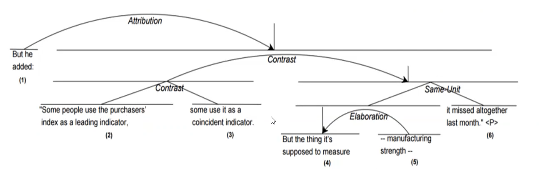
\includegraphics[width=0.8\linewidth]{comp550/rst-tree.png}
    \caption{RST Tree from Joy et al. (2013)}%
    \label{fig:rst-tree}
\end{figure}

applications using RST Tree features
\begin{itemize}
    \item essay grading
    \item automatic summarization
\end{itemize}

bootstrapping
\begin{itemize}
    \item gather discourse cues ``consequently'' $\to RESULT$
    \item supervised learn the discourse value
\end{itemize}


\subsubsection{Local Coherence Modelling}%
\label{ssub:local_coherence_modelling}

LCM (Barzilay and Lapata, 2005) looks at local cohesives in adjacent sentences

Generally, entity mentions follow patterns
\begin{itemize}
    \item first mention is often subject ``Maru is \ldots''
    \item mentions are clustered together ``\ldots Maru is grumpy. He likes cat food. \ldots (no more mentions)''
\end{itemize}

\textbf{entity grid} (Barzilay and Lapata, 2008)
\begin{itemize}
    \item plots entity mentions and syntactic role (see \ref{fig:entity-grid})
    \item extract features of document using relative freq of entity mention transition e.g. prob of subject $\to$ subject
    \item use to model ordering of a document, summary coherence, readability
\end{itemize}

\begin{figure}[ht]
    \centering
    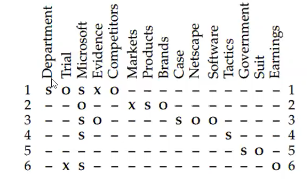
\includegraphics[width=0.5\linewidth]{comp550/entity-grid.png}
    \caption{Entity grid across 6 sentences (Bazilay and Lapata, 2008) with grammatical roles subject (s), object (o), or neither (x)}%
    \label{fig:entity-grid}
\end{figure}

entity grid extensions
\begin{itemize}
    \item combining global and local coherence (Elsner et al, 2007)
    \item other languages (Cheung and Penn, 2010)
    \item neural coherence (Nguyen and Joty, 2017)
    \item self-supervised (Xu et al, 2019)
        \begin{itemize}
            \item encode consecutive sentences $s, t$
            \item learn score using $s,t$ features
            \item SSL with NCE
        \end{itemize}
\end{itemize}

\section{Machine Translation}%
\label{sec:machine_translation}

\subsection{Introduction}%
\label{sub:introduction}

\subsubsection{Basics}%
\label{ssub:basics}

history
\begin{itemize}
    \item early optimisim using word-word and translation rules
    \item ALPAC report (1966) criticized MT prospects, AI winter
\end{itemize}

why is MT difficult
\begin{itemize}
    \item \textbf{lexical gaps} no 1-1 mapping between languages (e.g. dark blue)
    \item morphological e.g. number, tense
    \item syntactic e.g. word order
    \item semantic e.g. spatial relations
    \item pragmatic e.g. politeness, presupposition (e.g. again)
\end{itemize}

\textbf{Sapir-Whorf} hypothesis: the language you speak affect your thoughts
\begin{itemize}
    \item \textit{strong}: language determines and constrains all actions and thoughts
    \item \textit{weak}: language may influence action and thoughts
    \item e.g. Kuuk Thaayore use NESW instead of up-right-down-left
\end{itemize}

\subsubsection{Evaluation}%
\label{ssub:evaluation}

BLEU (Papieni et al, 2002) uses precision-oriented n-gram overlap
\begin{itemize}
    \item check if each $n$-gram in proposed translation is also in reference
    \item geometric mean over different $n$
    \item additional brevity penalty to account for common, short words
\end{itemize}

\subsubsection{Vauqouis Triangle}%
\label{ssub:vauqouis_triangle}

Vauquois triangle visually distinguishes MT systems (\ref{fig:vauquois})
\begin{itemize}
    \item direct
    \item syntactic
    \item semantic
    \item \textbf{interlingua} conceptual space common to all languages
\end{itemize}
\begin{figure}[h]
    \centering
    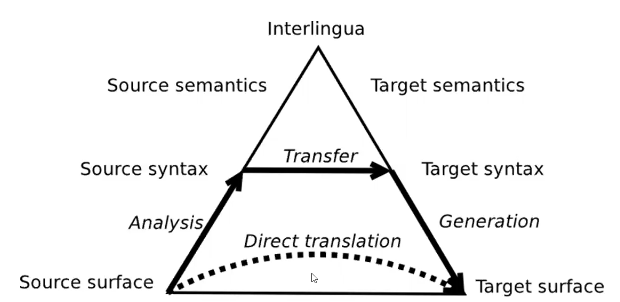
\includegraphics[width=0.8\linewidth]{comp550/vauquois.png}
    \caption{Vauquois Triangle}%
    \label{fig:vauquois}
\end{figure}



\subsection{Statistical MT}%
\label{sub:statistical_mt}

\subsubsection{Word-level}%
\label{ssub:word_level}

\textbf{noisy channel model} $E^* = \argmax_E P(E) P(F|E)$
\begin{itemize}
    \item assume target language $F$ is noisy encoded source $E$
    \item learn a language model $P(E)$ and translation model $P(F|E)$
\end{itemize}

MT as \textbf{alignment} between source and target sentence
\begin{itemize}
    \item get a parallel corpus e.g. novels, translated government docs
    \item first \textbf{sentence alignment}
        \begin{itemize}
            \item define similarity function using heuristics: length, cognate words, common subsequence
            \item search for optimal alignment using DP (e.g. edit distance $\to$ dynamic time warping)
        \end{itemize}
    \item then \textbf{word alignment}: plausibility, many-to-many mapping, word-order
    \item represent alignment as transform indices
\end{itemize}

\subsubsection{IBM Models}%
\label{ssub:ibm_models}

\textbf{IBM Model 1} maps source to target + NULL, assumes
\begin{itemize}
    \item each source word aligned to 0 or 1 targets
    \item don't model distortions of word order
    \item don't model likelihood of \textbf{fertility} phrase-level translation e.g. ``take a walk''
\end{itemize}

Model 1 learn by marginalizing over alignment $P(F|E) = \sum_A P(F|E,A) P(A|E)$
\begin{itemize}
    \item uniform translation length $P(A)$
    \item uniform probability of alignments $P(A|E)$
    \item word-level $P(F|E,A) = \prod_j P(f_j|e_{a_j})$ e.g. prob of word translation
\end{itemize}

learn $P(A|E,F),P(f|e)$ without existing alignments using EM
\begin{itemize}
    \item initialize randomly (in practise, not uniform)
    \item \textbf{E} use $P(f|e)$ params to compute $P(A|E,F) = \frac{P(F,A|E)}{\sum_A P(F,A|E)}$
    \item \textbf{M} given $P(A|E,F)$ update $P(f|e) = \frac{\sum_A P(A|e,f)}{Count(e)}$ to maximize
\end{itemize}

\textbf{IBM Model 2-5}
\begin{itemize}
    \item 2 does not assume equiprobable alignments e.g. prior of no crossing
    \item 3 models fertility (number of words needed to translate a word)
    \item 4,5 makes alignments depend on each other e.g. $P(F,A|E)$ as HMM seq labelling
\end{itemize}

\subsubsection{Phrase-level}%
\label{ssub:phrase_level}

translate phrases as units
\begin{itemize}
    \item can account for \textbf{idioms} e.g. ``coup de foudre'' $\to$ ``love at first sight''
    \item also benefits non-constituents e.g. ``Spass am'' $\to$ ``fun with the''
    \item learn a \textbf{phrase table} by looking at word co-occurrence
\end{itemize}

phrase-based MT $P(F|E) = \prod_n P(fp_n|ep_n) d(dist_n)$
\begin{enumerate}
    \item split sentence into phrases $E = ep_1,ep_2 \ldots$
    \item translate each phrase $P(fp | ep)$
    \item reorder phrases with penalty $d(dist)$
\end{enumerate}

\textbf{Greedy Hill Climbing} (Germann et al, 2001) \textbf{decoding} to search for best translation
\begin{enumerate}
    \item create initial complete candidate translation
    \item apply change operations to get a new candidate
        \begin{itemize}
            \item change translation of a word/phrase
            \item combine two words into phrase
            \item split up phrase into two sub-phrases
            \item rearrange translation
        \end{itemize}
    \item evaluate $P(E)P(F,A|E)$ and choose better
    \item iterate
\end{enumerate}

\subsection{Neural MT}%
\label{sub:neural_machine_translation}

\subsubsection{Neural Mechanisms}%
\label{ssub:neural_mechanisms}

\textbf{Neural Network Joint Models} (Delvin et al, 2014) replace components of statistical MT with neural
\begin{itemize}
    \item use traditional word alignment to get $\Sigma_i$ subsequence of $S$ useful for translating $t_i$
    \item predict output translation given input and previous translation decisions $P(T|S) = \prod_i P(t_i | t_{i-1} \ldots t_{i-n+1},\Sigma_i)$
    \item 2-layer FF + softmax predicts next word $t_i$
\end{itemize}

\textbf{Sequence-to-sequence} RNNs (Cho, 2014)
\begin{itemize}
    \item encode sequence with LSTM into $z$
    \item decode $z$ with LSTM (greedy or beam) into translation sequence $w^(t) | w^(s)$
\end{itemize}

\subsubsection{Attention}%
\label{ssub:attention}


\textbf{Attention} (Bahadanau et al, 2015) translates and soft aligns simultaneously
\begin{itemize}
    \item during decoding, take weighted combination of \textit{encoder} hidden as input $c_i = \sum \alpha_{ij} h_j$
    \item get energies $\alpha_{ij} = a(s_{i-1},h_j)$ using NN between decoder hidden and encoder hidden
    \item softmax normalize energies to get \textit{attention} weights $\alpha_{ij} = softmax(e_{ij})$
\end{itemize}

General attention is a \textit{soft} retrieval using query and (key,value)
\begin{itemize}
    \item \textbf{query} what we're looking for (current hidden)
    \item \textbf{key} representation of entry in memory (source word hidden)
    \item \textbf{value} information (source word hidden)
\end{itemize}

\subsubsection{Modern Tricks}%
\label{ssub:modern_tricks}

words as main units have issues
\begin{itemize}
    \item OOV
    \item morphologically rich e.g. Russian affix
    \item languages with compound words e.g. German
    \item named entities
\end{itemize}

character-level models lose semantic info and have very long sequence length

\textbf{Byte-Pair Encoding} (Sennrich et al, 2016) uses subword units
\begin{enumerate}
    \item start with character set as vocabulary
    \item compute frequency of vocab pairs
    \item add most common pair as new vocab item
    \item iterate
\end{enumerate}

\textbf{Backtranslation} (Sennrich et al, 2016) adds parallel training data from monolingual data
\begin{enumerate}
    \item use parallel to train a backward model from $T \to S$
    \item use backward model to get synthetic translations from monolingual $T$
    \item train full model on original + synthetic parallel $S \to T$
\end{enumerate}






\section{Summarization}%
\label{sec:summarization}

\subsection{Overview}%
\label{sub:automatic_summarization}

\textbf{text summarization} shortening source text into a \textit{text} summary
\begin{itemize}
    \item news headline from article
    \item movie reviews into critical consensus
\end{itemize}

purposes
\begin{itemize}
    \item \textbf{informative} replace source text (aggregate of reviews)
    \item \textbf{indicative} help decide whether to read source text (news headline)
    \item \textbf{critical} opinion of source text (movie summary to critical review)
\end{itemize}

methods
\begin{itemize}
    \item \textbf{extractive} copy and paste source text
    \item \textbf{abstractive} generate novel text
    \item \textbf{*pseudo-abstractive} combines extracts in novel ways
\end{itemize}

focus
\begin{itemize}
    \item \textbf{generic} no POV
    \item \textbf{user/query-focused} reflects goals/priority of query/user
\end{itemize}

source
\begin{itemize}
    \item \textbf{single-document} is usually single-author/POV
    \item \textbf{multi-document} has more issues between documents
        \begin{itemize}
            \item conflicting information
            \item redundancy
            \item combining information
        \end{itemize}

\end{itemize}

level of reader background
\begin{itemize}
    \item \textbf{update summary} provides relative info
\end{itemize}


steps in summarization
\begin{enumerate}
    \item \textbf{analysis} of source text for important parts
    \item \textbf{transformation} of common/contradictory points, new inferences
    \item \textbf{synthesis} to make final summary
\end{enumerate}

\subsection{Evaluation}%
\label{sub:sum_evaluation}

evaluate
\begin{itemize}
    \item \textbf{summary content} accurate, covers important, non-redundant
    \item \textbf{linguistic quality} grammaticality, coherence
\end{itemize}


common evaluations
\begin{itemize}
    \item human judgement
        \begin{itemize}
            \item[+] holistic, doesn't require gold standard
            \item[-] expensive, not rigorous, not consistent, biased
        \end{itemize}
    \item \textbf{ROUGE} (Lin, 2004) recall of n-grams from gold standard summary
    \item \textbf{Pyramid Method} (Nenkova and Passonneau, 2004)
        \begin{enumerate}
            \item break down summaries/gold into structured content units (SCUs)
            \item match SCUs between output, gold
        \end{enumerate}
    \item extrinsic evaluation tests whether summaries are \textit{useful}
        \begin{itemize}
            \item improves learning i.e. quiz results (McCallum et al, 2012)
            \item speed of identifying documents (Dorr et al, 2005)
        \end{itemize}
\end{itemize}


\subsection{Single-document}%
\label{sub:single_document}

can be viewed as supervised ML with careful feature choices
\begin{itemize}
    \item lexical features like content words are not as important
    \item discourse features like position, cues, structure are more important
\end{itemize}

Lin and Hovy (1998) trained a supervised method using position/discours cues
\begin{itemize}
    \item for each sentence in gold abstract, find position with highest similarity in source
    \item different corpora use different positions (WSJ uses title, first sentence of first paragraph, first sentence of second paragraph \ldots)
    \item \textbf{lead baseline} using first sentences is a strong baseline especially for news
\end{itemize}

\textbf{TFIDF} (Salton, 1988) term frequency inverse document frequency looks at words common in document, rare overall
\begin{itemize}
    \item TF is the count of th word
    \item IDF is $\log \frac{\text{num docs in corpus}}{\text{num docs with term } t + 1}$
\end{itemize}

\textbf{topic signatures} Lin and Hovy (2000) compares term frequency $t_i$ for related $R$ (and unrelated $\neg R$) documents using binomial distribution

\begin{table}[h]
    \centering
    \label{tab:label}
    \begin{tabular}{c|c|c}
                    & $R$       & $\neg R$ \\ \hline
        $t_i$       & $O_{11}$  & $O_{12}$  \\ \hline
        $\neg t_i$  & $O_{11}$  & $O_{12}$
    \end{tabular}
\end{table}

\begin{itemize}
    \item characterize each row as a binomial distribution $b(k;n;\theta)$where success is related article
    \item if $t_i$ is not important to domain then likelihood of data is \\ $L(H_1) = b(O_{11}; O_{11} + O_{12}, p) \cdot b(O_{21}; O_{21} + O_{22}, p)$
    \item otherwise probability of $t_i$ varies between this domain and other \\
    $L(H_1) = b(O_{11}; O_{11} + O_{12}, p_1) \cdot b(O_{21}; O_{21} + O_{22}, p_2)$
\item likelihood ratio $- 2 \log \frac{L(H_1)}{L(H_2)} $ shows how important this term is to domain
\end{itemize}

\subsection{Multi-document}%
\label{sub:multi_document}

SumBasic (Nenkova and Vanderwende, 2005) uses redundancy to figure out important things and make sure summary is non-redundant
\begin{enumerate}
    \item compute unigram dist $p(w_i) = \frac{n_i}{N}$
    \item[] \textit{repeat until summary length reached}
    \item rank sentences by average word probability
    \item pick highest scoring sentence $S^{best}$ and add to summary
    \item downweight chosen words, for $w_j$ in $S^{best}$ update $p_{new}(w_j) = p_{old}(w_j)^2$
\end{enumerate}

improvements
\begin{itemize}
    \item global optimum set of sentences instead of greedy
    \item account for similarities between bigrams
    \item avoid pronouns (if those pronouns aren't described)
    \item removing words from summary like ``therefore''
    \item modelling coherence of summary
\end{itemize}

Conroy et al (2006) combines topic signature method, non-redundancy module, and removes extra phrases:
\begin{itemize}
    \item gerund clauses e.g. I went to the store, \textit{skipping on a leg}
    \item restricted relative-clause appositives e.g. Bob, \textit{who is president}, disagreed
    \item attribution in a sentence e.g. Don't go, \textit{she said}, to the store
    \item lead adverbs e.g. \textit{Hopefully}, we find a solution
\end{itemize}


Neural methods made possible by large datasets of news and summaries (CNN, NYT, Newsroom) cast as a supervised learning problem or even RL optimizing ROUGE where actions are selecting summary sentences.

\section{Natural Language Generation}%
\label{sec:natural_language_generation}

requires selecting
\begin{itemize}
    \item appropriate content
    \item appropriate form to express it
\end{itemize}

generation
\begin{itemize}
    \item
    \item \textbf{text-to-text}
\end{itemize}

\subsection{Data-to-Text}%
\label{sub:data_to_text}

\textbf{data-to-text} formal to NL (reverse of NLU)

basic systems
\begin{itemize}
    \item \textbf{canned text} pre-written text at certain time
    \item \textbf{template filling} pre-generated template with variable slots
\end{itemize}

\subsubsection{Components}%
\label{ssub:components}

\begin{enumerate}
    \item \textbf{content selection} decide what to say
        \begin{itemize}
            \item application-specific doc analysis
        \end{itemize}
    \item \textbf{document structuring} how to structure output
        \begin{itemize}
            \item order of output (importance, coherence)
            \item e.g. \textit{argumentation theory} (Carenini and Moore, 2006)
        \end{itemize}
    \item \textbf{microplanning} of specific text to output
        \begin{itemize}
            \item selecting lexical items
            \item sentence planning of lexicals into clauses
            \item generate referring expressions e.g. Justin, him, PM
        \end{itemize}
    \item \textbf{surface realization} convert specific plan to output form
        \begin{itemize}
            \item depends on how specified discourse plan is
            \item e.g. \textbf{FUF/Surge} (Elhadad and Robin, 1996) cascade of deterministic rules from attrib-value matrix
            \begin{enumerate}
                \item map semantic to syntactic roles (agent $\to$ subject)
                \item syntactic alternations (active/passive, dative)
                \item fill in defaults for underspecification (NPs are definite)
                \item handle closed-class words (personal pronoun, feminine $\to$ she)
                \item order components (subject, verb, indirect object, direct object)
                \item fill in inflections (he, to hand $\to$ he hands)
                \item linearize the tree into the final string
            \end{enumerate}
        \end{itemize}
\end{enumerate}


\subsection{Text-to-Text}%
\label{sub:text_to_text}

generation changing something from source to target
\begin{itemize}
    \item language, MT
    \item length, summarization
    \item complexity, text simplification
    \item style, style transfer
\end{itemize}

\subsubsection{Integer Linear Programming}%
\label{ssub:integer_linear_programming}

\textbf{sentence fusion} combines information from multiple sentences
\begin{itemize}
    \item equivalent to summarization
\end{itemize}

graph sentence fusion
\begin{enumerate}
    \item generate \textbf{sentence graph} (\ref{fig:sentence-graph}) merging sentences' dependency trees
    \item select subset of nodes and extract a new sentence following constraints (important words, relations, output length \ldots)
\end{enumerate}

\begin{figure}[ht]
    \centering
    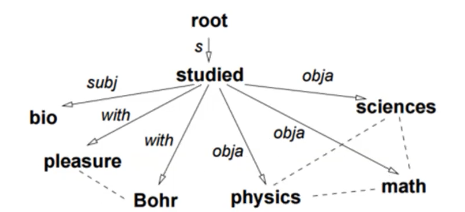
\includegraphics[width=0.6\linewidth]{comp550/sentence-graph.png}
    \caption{Sentence Graph (Filippova and Strube, 2008) for ``He studied science with pleasure''+``He studied math and physics with Bohr''}
    \label{fig:sentence-graph}
\end{figure}

\textbf{integer linear programming} where all constraints, objectives are linear functions of integers
\begin{itemize}
    \item make binary selection variable $x_{hw}^{l}$ for each edge in sentence graph from $h$ to $w$ with label $l$
    \item optimize $\sum_x x_{hw}^{l} P(l|h) I(w)$ with grammaticality $P$, importance $I$, and constraints
    \item each word has at most one head $\forall w \in W, \sum x_{hw}^l \leq 1$
    \item selected nodes form connected tree $\forall w \in W, \sum x_{hw}^l - \frac{1}{|W|}\sum x_{wu}^l \geq 0$
\end{itemize}

ILP can accomodate more constraints
\begin{itemize}
    \item allows \textbf{declaritive} spec of objectives/constraints
    \item can be solved efficiently with off-the-shelf solvers
\end{itemize}

\subsubsection{Modern Methods}%
\label{ssub:modern_methods}

using condition language model $P(x^{t+1} | source, x^{1 \ldots t})$

handling OOV, named entities
\begin{itemize}
    \item sub-word representations (e.g. WordPiece)
    \item copy mechanism to copy from input sequence
\end{itemize}

correctness in generation
\begin{itemize}
    \item $\sim 30\%$ of neural generated text have factual errors
    \item post-editing model to detect and correct errors (Cao et al, 2020)
\end{itemize}

controllable text generation
\begin{itemize}
    \item ensure output style, politeness, goal, etc.
\end{itemize}


\section{Evaluation}%
\label{sec:evaluation}

\subsection{Measures}%
\label{sub:measures}
\textbf{automatic} measures don't require human effort


classes of measures
\begin{itemize}
    \item \textbf{intrinsic} pertains to the exact task we're solving (perplexity for LM)
    \item \textbf{extrinsic} petrains to downstream task (MT for LM)
\end{itemize}


eval \textbf{validity} is whether improving the measure means real progress in our model
\begin{itemize}
    \item \textbf{internal validity} is study conclusion warranted?
        \begin{itemize}
            \item are comparisons fair? (training data, model size)
            \item confounding factors
        \end{itemize}
    \item \textbf{external validity} do study conclusions generalize to other data/situations?
        \begin{itemize}
            \item size of the test data
            \item is setup biased towards certain models?
            \item \textbf{domain adaptation} generalizes across domains
        \end{itemize}
    \item \textbf{construct validity} do evaluations measure what they claims to?
        \begin{itemize}
            \item does ROUGE reflect usefulness of summaries?
            \item does better PPL lead to lower word error rate in ASR?
            \item does lower word error rate lead to better satisfaction with ASR systems?
        \end{itemize}
\end{itemize}

We want cheap, automatic measures that correlate with gold standard (human) measures of NLP

\subsection{Turing Test}%
\label{sub:turing_test}

Does a machine exhibit intelligent behaviour?
\begin{itemize}
    \item human interlocutor chats with an agents A and B through text interface
    \item after 5 minutes must decide which is human and which is machine
\end{itemize}

Competitions organized to approximate
\begin{itemize}
    \item Loebner Prize annual competition copies format of TT
    \item Reading University
    \item Alexa Prize inspired by TT
\end{itemize}

Most winning systems do not approximate human intelligence but rather deceive their evaluators
\begin{itemize}
    \item Eugene Goostman 13 y/o Ukranian boy ???
    \item Rose (Loebner 2014 winner)
\end{itemize}

\textbf{Goodhart's Law} once a measure of some quality is turned into a target to optimize, it is no longer a good measure of quality
\begin{itemize}
    \item some ``tricks'' do not represent genuine progress
    \item for ROUGE: using entire word length, using more content words etc \ldots
\end{itemize}

\subsection{Winograd Schema Challenge}%
\label{sub:winograd_schema_challenge}

Issues with evaluation
\begin{itemize}
    \item uncommon, systematic issues can be ignored using standard test sets
    \item \textbf{``cheap tricks''} of statistical systems can get the answer right for the wrong reason (Levesque, 2013)
        \begin{itemize}
            \item QA systems using regularities in patterns to retrieve memorized knowledge
            \item Summarization using extraction and redundancy without understanding
        \end{itemize}
\end{itemize}

\textbf{Winograd Schema Challenge} multiple-choice questions that require deeper understanding
\begin{itemize}
    \item Joan thanks Susan for all the help \textit{she} had given/received
    \item Knowledge Hunting (Emami et al, 2018) parse, extract, search on web and find similar examples
    \item Pretrained LM looking at which sentence is likelier for WSC (Trinh et al, 2018; Devlin et al, 2018)
\end{itemize}

Statistical workarounds still exist
\begin{itemize}
    \item predictable structure ``predicate because predicate``
    \item limited test size (273)
    \item associativity (``building'' closer to ``famous'' than ``map'')
\end{itemize}

Switch antecedents as a new evaluation protocol (Trichelair et al, 2019)
\begin{itemize}
    \item ``Emma/Janie'' did not pass the ball to ``Janie/Emma''
    \item check whether models are consistent across switches!
    \item models do better on associative subset
\end{itemize}

\subsection{Bias}%
\label{sub:bias}

Machine learning systems learn biases inherent in data
\begin{itemize}
    \item our \textit{world} has negative biases
    \item learned methods can produce even more biased results than the data
    \item training objectives incentivise systems to guess most common class when uncertain
\end{itemize}

General debiasing algorithms, RBA (Zhao et al, 2017)
\begin{itemize}
    \item identify axis of bias (e.g. gender, race, religion)
    \item add optimization constraints to be within margin of desired bias
\end{itemize}























\end{document}
